\chapter{SMTP Configuration}

Obidos uses the SMTP configurations for sending email to users for various purposes.
For example, the admin can chose to send email confirmation for new user account.
When a user shares an Item with another user, an email is sent to the beneficiary.
In order to send emails, Obidos needs information about the SMTP server.
\textcolor{red}{Only one SMTP Configuration can be created per Obidos instance.}

\section{Create New SMTP Configuration}

From the top level "Settings" menu select "Create SMTP Settings".

\begin{figure}[H]
\centering
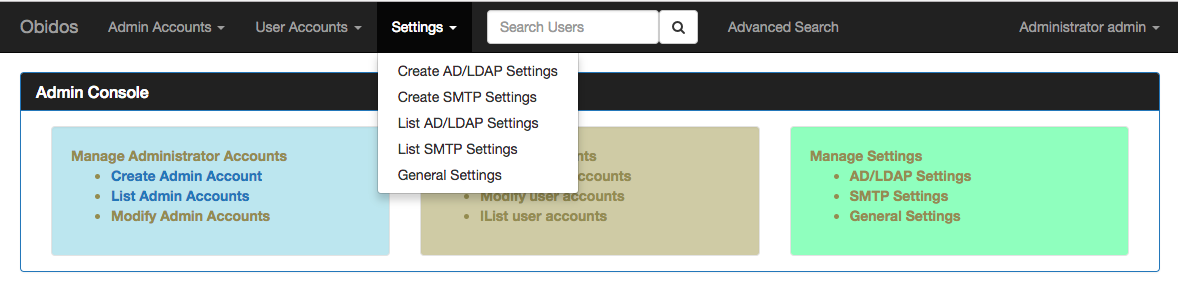
\includegraphics[width=90mm]{admin/Settings-Menu.png}
\caption{Create New SMTP Configuration}
\label{fig: Figure}
\end{figure}

The fields of the Configuration are as shown in the following figure.

\begin{figure}[H]
\centering
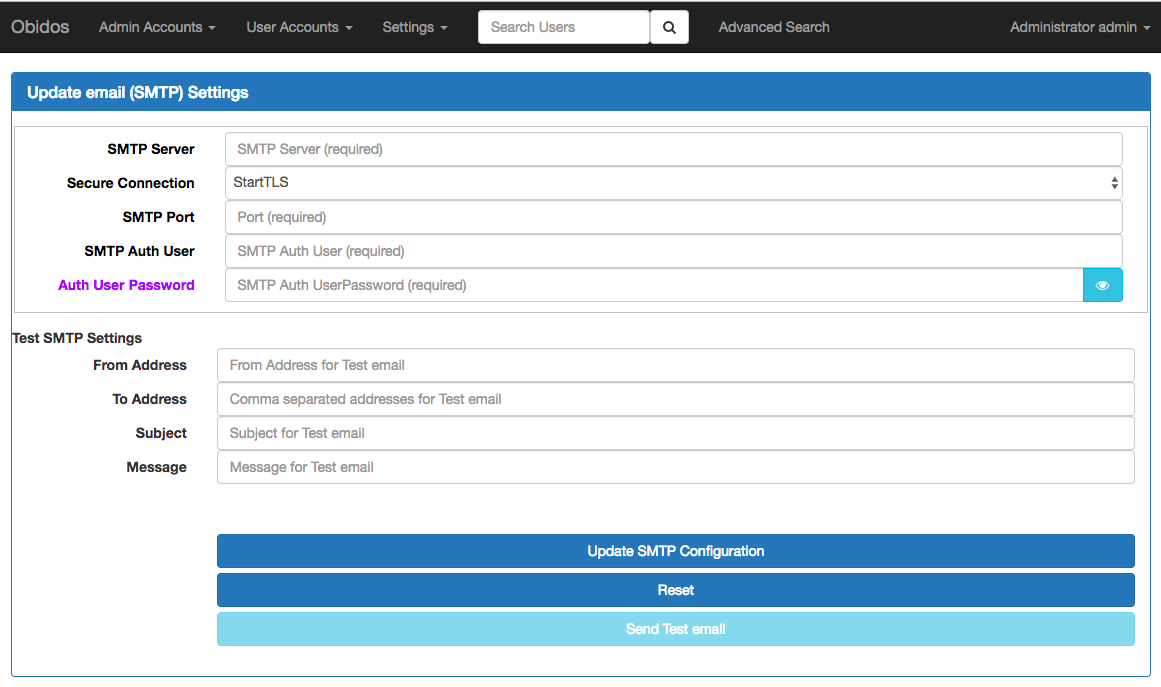
\includegraphics[width=90mm]{admin/SMTP-Details.png}
\caption{SMTP Configuration Fields}
\label{fig: Figure}
\end{figure}

The SMTP Server field is the fully qualified hostname of the server.

The "Secure Connection" field can be StartTLS or SSL or 'Not Secure'.

SMTP Port is the TCP/IP port on which the mail server (MTA) is listening for incoming connections.
Traditionally, for Non-secure connections this is 25.
Implicit encrypted (i.e., SSL or TLS) SMTP uses port 465.
StartTLS popularly uses port 587.

SMTP Auth User is the account using which authentication is done to the mail server.

The password for this account should be provided in the field "Auth User Password".
\section{List SMTP Configuration}

From the top level "Settings" menu select "List SMTP Settings".

\begin{figure}[H]
\centering
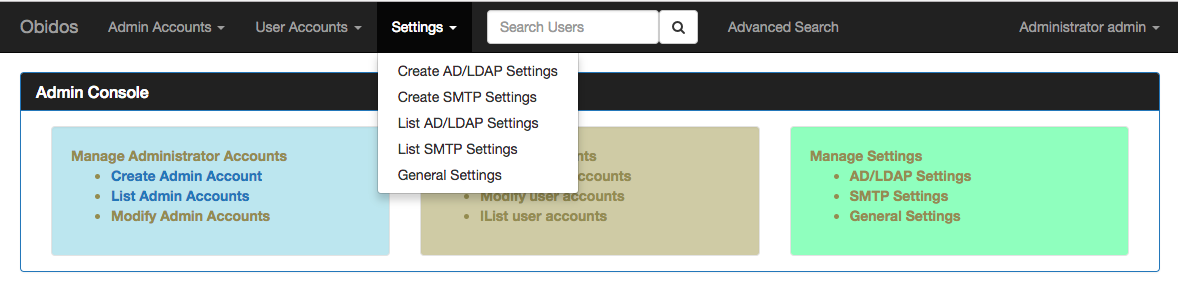
\includegraphics[width=90mm]{admin/Settings-Menu.png}
\caption{List SMTP Configuration}
\label{fig: Figure}
\end{figure}

\section{Edit SMTP Configuration}

From the top level "Settings" menu select "List SMTP Settings".
The result will be as shown in the following figure.

\begin{figure}[H]
\centering
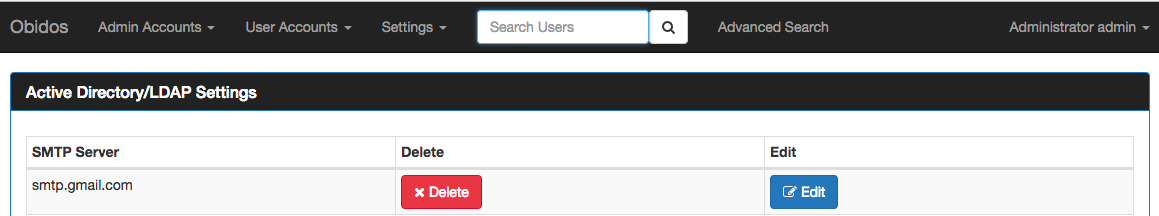
\includegraphics[width=90mm]{admin/SMTP-Edit.png}
\caption{Edit SMTP Configuration}
\label{fig: Figure}
\end{figure}

Click on the "Edit" button and the screen will show the existing details.
